https://mcs-notes2.open.ac.uk/files/m337dq.pdf

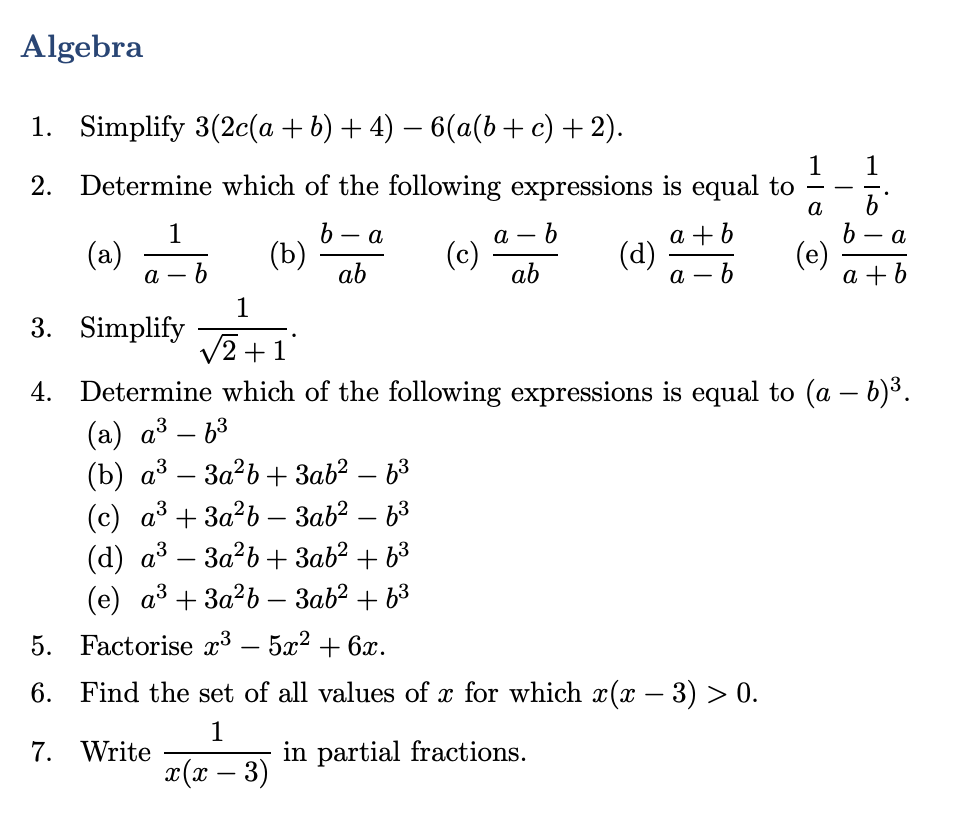
\includegraphics[width=400pt]{img/ou-entry-2236.png}

\begin{enumerate}
\item
\begin{align*}
  3(2ac + 2bc + 4) - 6(ab + ac + 2)
  &= 6ac + 6bc + 12 - 6ab -6ac -12 \\
  &= 6bc - 6ac \\
  &= 6c(b-a)
\end{align*}
\item (b)
\item
 \begin{align*}
    \frac{1}{\sqrt{2} + 1}
   &= \frac{\sqrt{2} - 1}{(\sqrt{2} + 1)(\sqrt{2} - 1)} \\
   &= \sqrt{2} - 1
 \end{align*}
\item (b)
\item
\begin{align*}
  x(x^2 - 5x + 6) = x(x-2)(x-3)
\end{align*}
\item \begin{align*}
        y &= x(x - 3) \\
          &= x^2 - 3x
      \end{align*}
      Second derivative is positive.
      $y > 0$ for $x \in (-\infty, 0) \cup (3, \infty)$.
\item \begin{align*}
        \frac{1}{x(x - 3)} &= \frac{A}{x} + \frac{B}{x-3} \\
        1                  &= Ax - 3A + Bx \\
        A &= -1/3 \\
        B &= 1/3 \\
        \frac{1}{x(x - 3)} &= \frac{-1}{3x} + \frac{1}{3(x - 3)}
      \end{align*}
      Check:
      \begin{align*}
        \frac{-1}{3x} + \frac{1}{3(x - 3)}
        &= \frac{-3(x - 3) + 3x}{9x(x - 3)} \\
        &= \frac{9}{9x(x - 3)} \checkmark
      \end{align*}



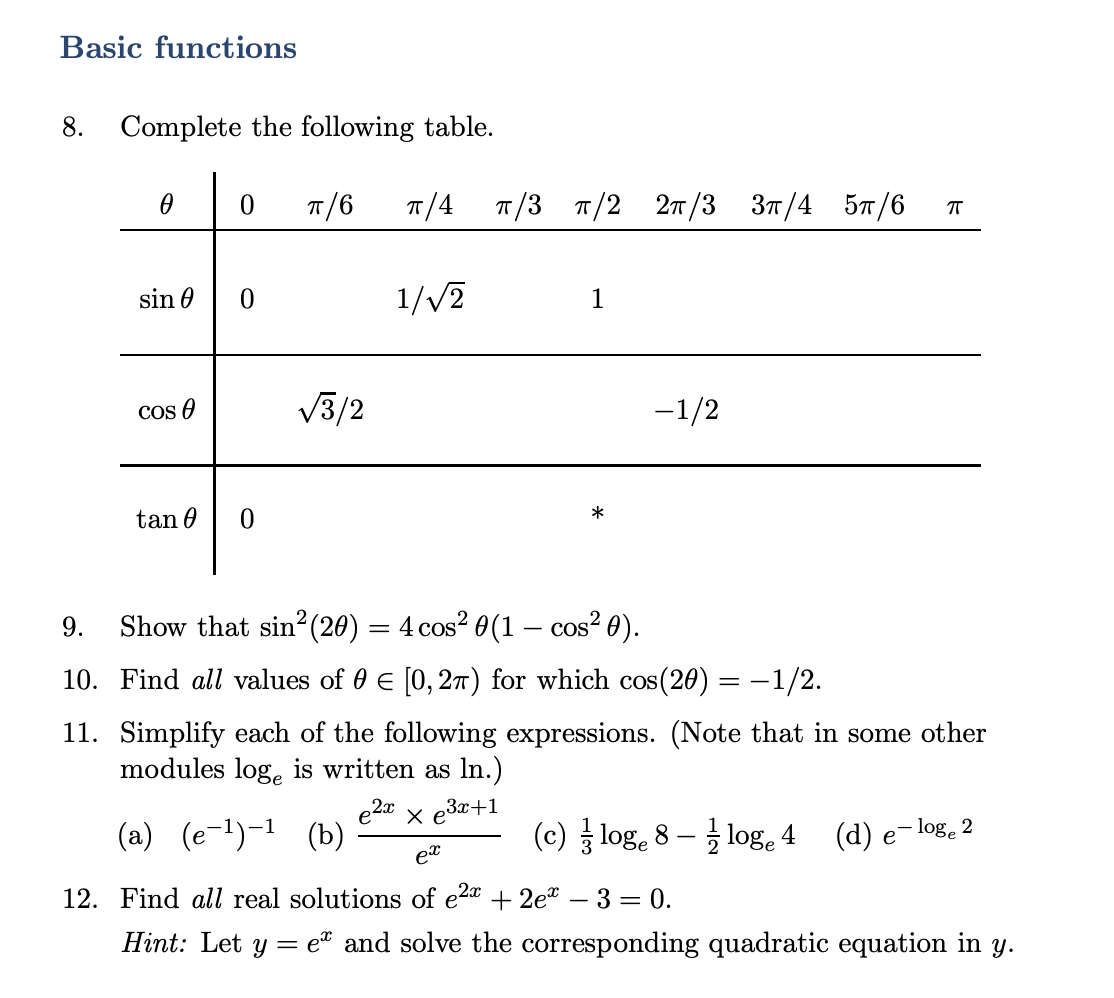
\includegraphics[width=400pt]{img/ou-entry-9439.png}

\begin{enumerate}
\item
  \begin{table}[h!]
    \centering
    \begin{tabular}{c|ccccccccc}
      $\theta$      & 0 & $\pi/6$      & $\pi/4$      & $\pi/3$     & $\pi/2$  & $2\pi/3$      & $3\pi/4$        & $5\pi/6$      & $\pi$ \\
      \hline
      $\sin \theta$ & 0 & 1/2          & $1/\sqrt{2}$ & $\sqrt{3}/2$ & 1        & $\sqrt{3}/2$ & $1/\sqrt{2}$    & 1/2           & 0\\
      $\cos \theta$ & 1 & $\sqrt{3}/2$ & $1/\sqrt{2}$ & 1/2          & 0        & -1/2         & $-1/\sqrt{2}$   & $-\sqrt{3}/2$ & -1\\
      $\tan \theta$ & 0 & $1/\sqrt{3}$ & 1            & $\sqrt{3}$   & $\infty$ & $-\sqrt{3}$  & -1              & $-1/\sqrt{3}$ & 0
    \end{tabular}
  \end{table}
\end{enumerate}
\item \begin{align*}
    \sin^2(2\theta)
    &= (2\sin\theta\cos\theta)^2 \\
    &= 4\cos^2(1-\cos^2\theta)
  \end{align*}
\item $\cos(2\theta) = -1/2$ implies $2\theta = 4\pi/6$ or $2\theta = 8\pi/6$, i.e. $\theta \in \{\pi/3, 2\pi/3 \}$.
\item
  \begin{enumerate}[label=(\alph*)]
  \item $e$
  \item \begin{align*}
          \frac{e^{2x}e^{3x+1}}{e^x} = e^xe^{3x+1}
        \end{align*}
  \item \begin{align*}
      \frac{1}{3} \log_e 8 - \frac{1}{2} \log_e 4
      &= 3 \cdot \frac{1}{3} \log_e 2 - 2 \cdot \frac{1}{2} \log_e 2 \\
      &= 0
    \end{align*}
  \item \begin{align*}
      e^{-\log_e 2} = 1/2
    \end{align*}
  \end{enumerate}
\item \begin{align*}
    e^{2x} + 2e^x - 3 = 0
  \end{align*}
  Let $y = e^x$. Then we have
  \begin{align*}
    y^2 + 2y - 3   &= 0 \\
    (y + 3)(y - 1) &= 0
  \end{align*}
  hence $e^x = -3$ or $e^x = 1$,

  hence the only real solution is $x = \ln 1$.
\end{enumerate}

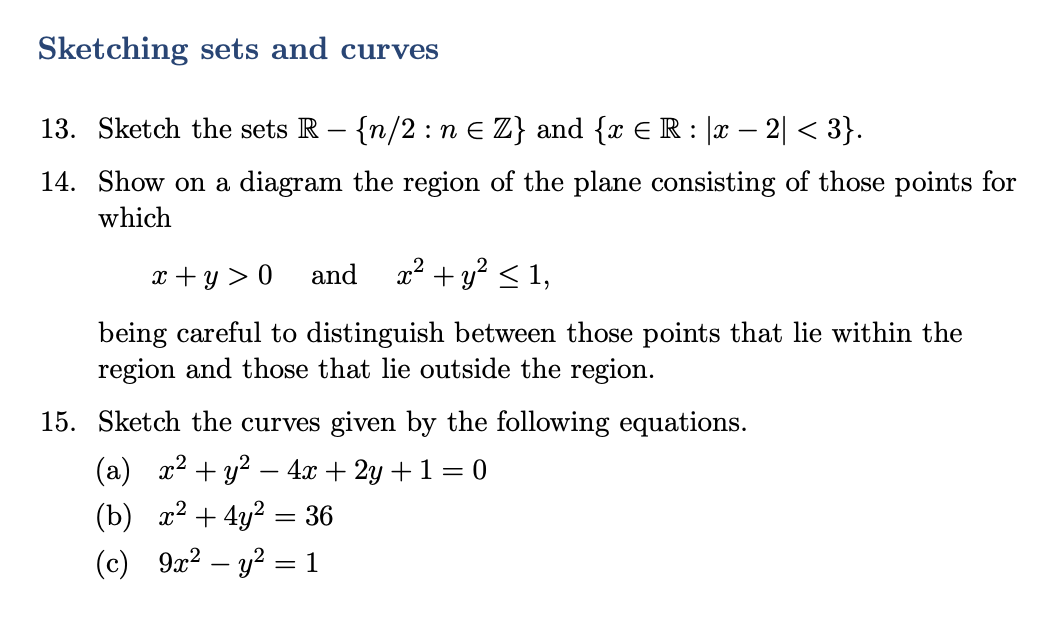
\includegraphics[width=400pt]{img/ou-entry-cdc6.png}


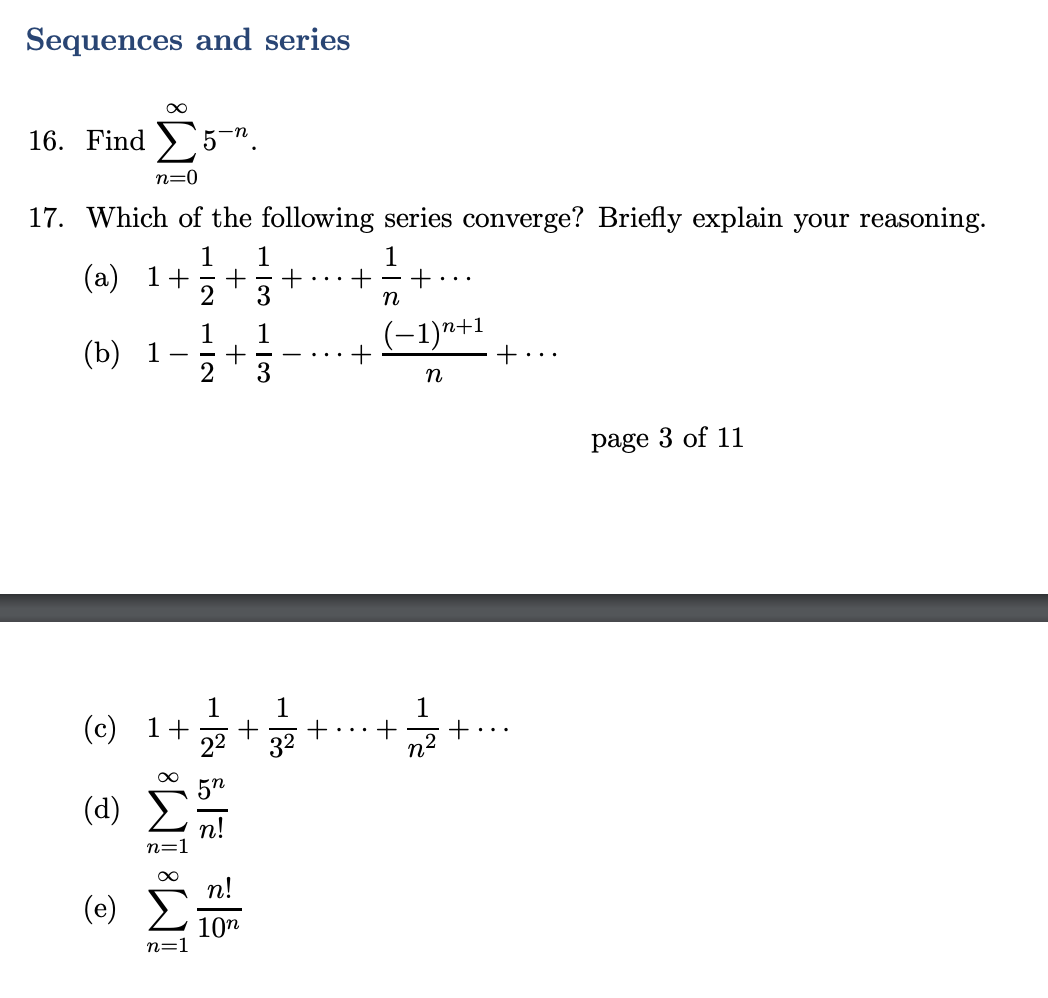
\includegraphics[width=400pt]{img/ou-entry-ce7c.png}
\begin{enumerate}
\item \begin{align*}
    \sum_{n=0}^\infty \Big(\frac{1}{5}\Big)^n
  \end{align*}
  Geometric series formula...how to derive?
\item
  \begin{enumerate}[item=(\alph*)]
  \item Ratio test:
    \begin{align*}
      \lim_{n\to\infty} \frac{1/(n+1)}{1/n}
      &= \lim_{n\to\infty} \frac{n}{n+1} \\
      &= \lim_{n\to\infty} \frac{1}{1 + 1/n} \\
      &= 1
    \end{align*}
    Inconclusive by the ratio test.

    This is the harmonic series and it diverges.
  \item \begin{align*}
      \frac{(-1)^{n+2}}{n+1} / \frac{(-1)^{n+1}}{n}
      &= \frac{(-1)^{n+2}n}{(-1)^{n+1}(n+1)} \\
      &= (1 + n)(-1) < 0
    \end{align*}
    Converges by Alternating Series test.
  \end{enumerate}
\item Ratio test:
  \begin{align*}
      \lim_{n\to\infty} \frac{1/(n+1)^2}{1/n^2}
      &= \lim_{n\to\infty} \frac{n^2}{n^2 + 2n + 1} \\
      &= \lim_{n\to\infty} \frac{1}{1 + 2/n + 1/n^2} \\
      &= 1
    \end{align*}
    Inconclusive. This converges; every term is smaller than harmonic series.

\end{enumerate}


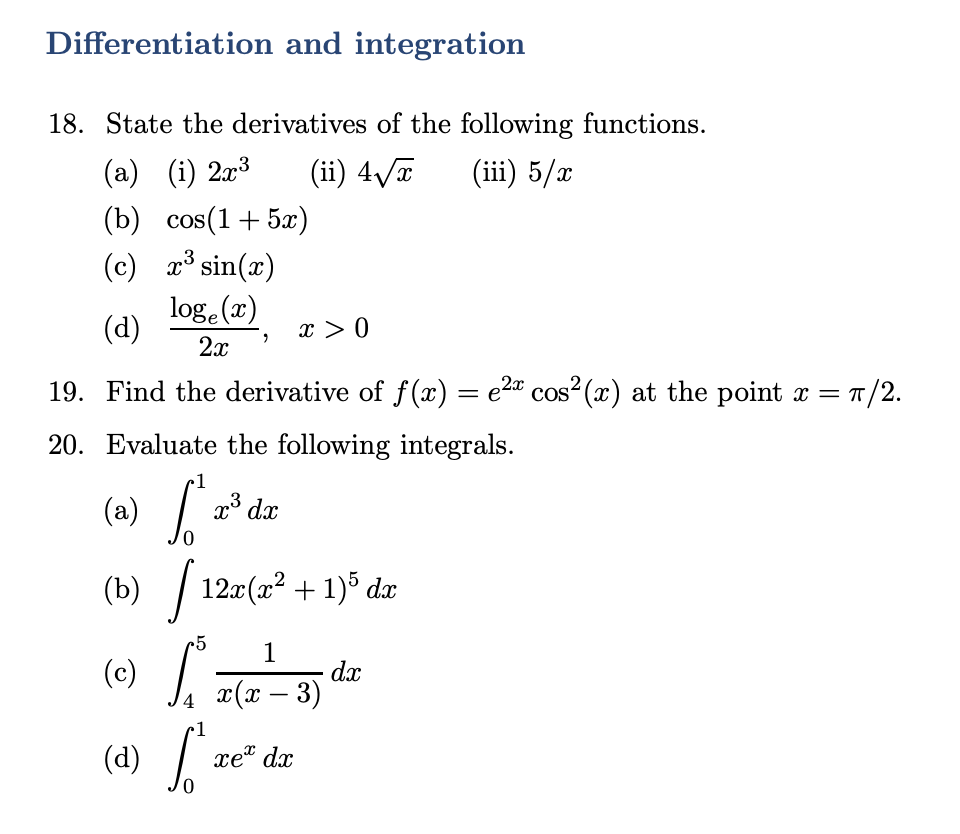
\includegraphics[width=400pt]{img/ou-entry-a82d.png}



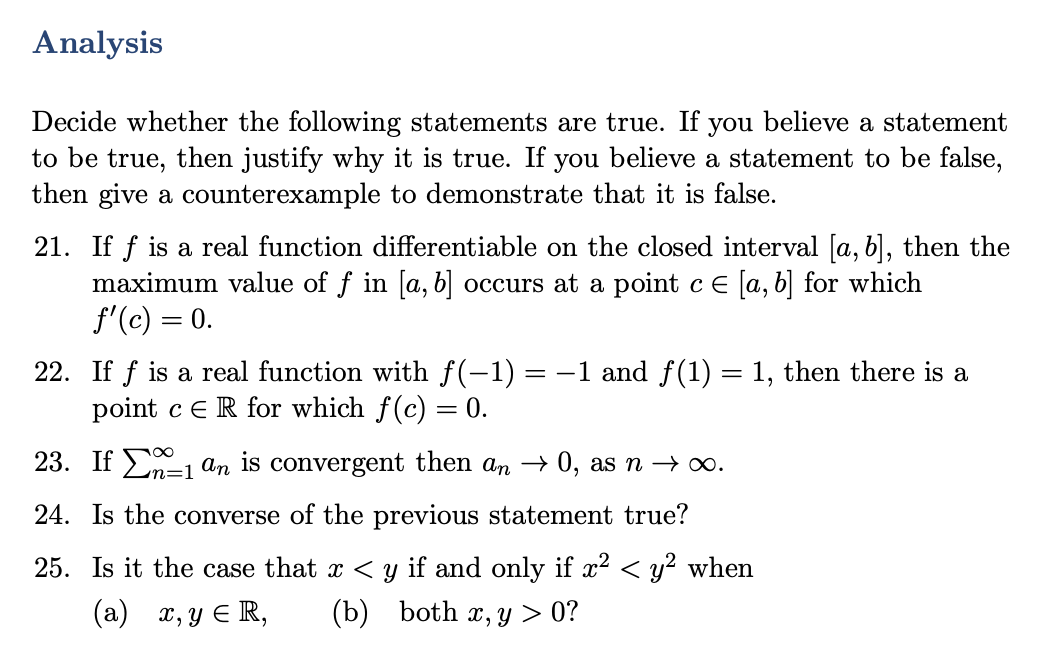
\includegraphics[width=400pt]{img/ou-entry-efb5.png}

\begin{enumerate}
\item False. E.g. the maximum of $f(x) = x$ occurs at $b$ and yet $f'(b) = 1$.
\item False. This is only true if $f$ is continuous. Counter-example
  \begin{align*}
    f(x) =
    \begin{cases}
      -1 &~~~\text{if}~~~ x <= 0\\
      1 &~~~\text{if}~~~ x > 0
    \end{cases}
  \end{align*}
\item
\end{enumerate}
